\chapter{Создание ПО для статического анализа кода системы компьютерной верстки TeX}

Необходимость создания специализированного программного обеспечения обусловлена необходимостью в оптимизации процесса проверки нормкотроля документов посредством человеческих усилий. За время наблюдения за процессом проверки работ на нормконтроль были замечены следующие моменты:

\begin{enumerate}
    \item каждый человек проверяет определенные моменты в силу своих знаний;
    \item каждый человек имеет разную длительность проверки;
    \item каждый человек может ошибаться в моментах проверки или же их пропускать.
\end{enumerate}

Конечным продуктом проверки является \guillemotleftудостоверение\guillemotright\verb| |о ее прохождении. Ввиду выше перечисленных моментов можно отметить, что у разных документов могут остаться различные ошибки и неточности, пропущенные или не проверенные конкретным человеком. Таким образом на представление общественности попадает недоделанный документ различной степени ошибочности, что является грубым нарушением правил нормконтроля и допуска к сдаче работы.

Разработанная программа позволит за короткое время проанализировать документ и предоставить информацию о неверном оформлении на основе заранее заданного шаблона и ожидаемых характеристик.

\section{Создание файла конфигурационных характеристик}

Ввиду того, что у каждого отдельно взятого учреждения или организации могут быть свои дополнительные правила по оформлению документов, наложенные или замещающие условно-общепринятые нормы, необходимо составить некоторый текстовый файл, который должен отображать требуемые для проверки характеристики. Данный файл должен создаваться отдельно под каждый различный тип оформления.

Файл должен иметь расширение \verb|.json| являющееся популярным и удобным для создания конфигурационных файлов. Рассмотрим каждую характеристику возможную конфигурационном файле. Если характеристики не обозначено в файле, то для нее применяется стандартное значение.

    Ссылки. Объект \verb|links| в файле содержит ключи относящиеся к настройке проверки ссылок конкретных элементов. Ключи описывают зарезервированные названия объектов среди, которых: \verb|figure|, \verb|equations|, \verb|table|, \verb|listings|, \verb|text|. Данные названия относятся к соответствующим аргументам команды \verb|\begin|: фигура, уравнение, таблица, листинг, а так же ссылки не выделенные в отдельный элемент. Ключ \verb|equations| (Листинг \ref{ls:01}) представляет собой внутреннюю структуру содержащую ключ \verb|position| принимающее в качестве значения массив содержащие резервированные слова \verb|before|, \verb|after|, которые означают возможность нахождение ссылки на элемент \verb|до| и \verb|после| нахождения данного элемента в тексте. Значение ключа \verb|caption| означает необходимость проверки на соответствие значения стоящего до ссылки текста, определяющее смысловое назначение ссылки на элемент. Ключ \verb|name| определяет необходимое имя для идентификации типов объектов ссылки. Ключ \verb|referToEverything| определяет необходимость ссылаться на каждый определенный элемент в тексте. 
    
    \begin{lstlisting}[caption = {Пример конфигурации ссылок}, label={ls:01}]
    "links" : {
      "equations": {
         "position" : ["before", "after"],  
         "caption" : ["Уравнение ", "уравнение "],
         "name" : "eq",
         "referToEverything" : true
      }
   }
    \end{lstlisting}

    Количество слов в названиях. Для того, чтобы давать наиболее полное представление о материале, находящемся в главах, параграфах и пунктах необходимо использовать распространённые предложения. Для отслеживания данного правила существует характеристика \verb|lengthOfNames|. Рассмотрим ключи и значения на примере Листинг \ref{ls:02}. Ключи \verb|chapter|, \verb|section|, \verb|subsection|, \verb|caption| соответствуют смысловым определениям: глава, параграф, пункт, подпись. Каждый из ключей представляет собой структуру. Такие структуры содержат ключи \verb|minLength| и \verb|minWordLength|, соответственно означающие минимальное допустимое количество слов в названии и минимальную допустимую длину засчитываемого слова.  
    
     \begin{lstlisting}[caption = {Пример конфигурации названий}, label={ls:02}]
    "lengthOfNames":{
      "chapter" : {
         "minLength" : 3,
         "minWordLength" : 3
      },
      "section" : {
         "minLength" : 4
      },
      "subsection" : {
         "minLength" : 3
      },
      "caption":{
         "minLength" : 3
      }
   }
    \end{lstlisting}

    Списки. Характеристика \verb|lists| определяет форматирование и использования списков и их объектов.  Рассмотрим ключи и значения на примере Листинг \ref{ls:03}. Ключи, представляющие собой структуры соответствуют названиям списков. Опишем ключи и их смысловые значения структур характеристики \verb|lists|. Ключ \verb|itemOptions| определяется массивом значений возможных для использования в опциях команды \verb|\item|, в случае значения \verb|null| запрещается использование опций у данной команды. Ключ \verb|itemFormatting| представляет структуру, содержащую массивы символов, рассмотрим их подробнее. Массив значений ключа \verb|firstLetter| определяет возможность использования заглавных букв при значении \verb|A| как начальной после команды \verb|\item|, и аналогично использования строчных букв в случае значения \verb|a|. Ключ \verb|endLetter| определяет массив значений символов, один из которых должен быть в конце описываемого \verb|item|. Ключ \verb|lastStringEndLetter| определяет массив значений символов, один из которых должен быть в конце описываемого последнего \verb|item| списка. Значение ключа \verb|enableAnotherLists| определяет возможность использования в документе иных типов списков, кроме описанных. 
    \begin{lstlisting}[caption = {Пример конфигурации списков}, label={ls:03}]
    "lists" :{
      "enumerate": {
         "itemOptions" : [null],
         "itemFormatting" :{
            "firstLetter" : ["A","a"],
            "endLetter" : [";"],
            "lastStringEndLetter" : ["."]
         }
      },
      "enableAnotherLists" : false   
   }
    \end{lstlisting}

    Ссылки на литературные источники. Данная характеристика описывается структурой \verb|biblioLinks| (Листитнг \ref{ls:04}). Структура отвечает за настройку форматирования и проверки ссылок на список литературы, описанный в файле с расширением \verb|.bib| и вызываемых по номеру в виде аргумента с помощью команды \verb|\cite|. Она содержит ключи с названиями  \verb|referBeforeSentenceEnd| и \verb|referToEverything|, соответственно означающие необходимость размещения ссылок до конца предложения, и необходимость использовать в тексте все ссылки на описанные литературные источники.
    
    \begin{lstlisting}[caption = {Пример конфигурации ссылок на литературные источники}, label={ls:04}]
    "biblioLinks" :{
          "referBeforeIndentStart" : true,
          "referToEverything" : true
       },
     \end{lstlisting}   

     Общее форматирование. Характеристика \verb|generalTextFormatting| содержит в себе смысловые ключи, которые не подходят для иных структур или представляют собой элементарную проверку. В качестве таких ключей выделяются \verb|useDashInsteadOfHyphen| означающий необходимость использовать тире вместо десисов между стоящих слов разделенных табуляцией и \verb|useGuillemotInsteadQuotationMarks| определяющий использования форматированных кавычек вместо обычных (Листинг \ref{ls:05}).

        \begin{lstlisting}[caption = {Пример общей конфигурации форматирования документа}, label={ls:05}]
     "generalTextFormatting" :{
      "useDashInsteadOfHyphen" : true,
      "useGuillemotInsteadQuotationMarks" : true
   }
     \end{lstlisting}   

\section{Подготовка файлов к статическому анализу}

Для начала проведения статического анализа, необходимо указать путь до архива с файлами расширения \verb|.tex| и иных файлов относящихся к документу, а так же путь до файла с расширением \verb|.json|, который будет является файлом характеристик и параметров проверки. 

После запуска программы и указания путей к файлам содержимого проводится валидация файла характеристик на предмет корректности данных, ключей и значений. Успешная валидация сопровождается заполнением соответствующих полей класса характеристик и позволяет перейти к следующему этапу работы программы -- формирование единого файла документа для удобного проведения анализа. 

Этап включает в себя нахождение задание пользователем начального файла, где содержится окружение  \verb|\begin{document}...\end{document}|, которое в свою очередь содержит все команды используемые для создания документа. В случае ошибки поиска пользователю должны выдаться инстукции по корректировке файлов, чтобы создать необходимую структуру в файле или же выбрать иной файл и повторно запустить программу. 

Нахождение команд  \verb|\begin{document}...\end{document}| позволяет однозначно найти точку входа и выхода программы, тем самым определяя, что весь текст и команды относящиеся к компиляции документа находятся между началом и концом \guillemotleftблока\guillemotright  \verb| document|.

После успешного нахождения окружения \verb|document| программа обрабатывает все команды внутри окружения. В случае если функционал команды отвечает за подключение файла, например в таких командах как \verb|\input{Путь до файла}| и \verb|\include{Путь до файла}|, происходит попытка открытия файла с расширением \verb|.tex| и поиска внутри команд верстки \LaTeX \, с последующей вставкой найденных команды вместо команды подключения файла. Завершение данного этапа предполагает получение программой массива элементов, содержащих различные данные о командах их свойствах, аргументах и параметрах, расположении и иных данных. Набор команд является основным элементом, с которым взаимодействуют функции анализа документа на предмет сопоставления заявленным характеристикам. 


\section{Проведение анализа загруженных пользователем файлов}

Синтаксический и лексический анализ является основой работы описанного выше этапа по единого текстового файла и в последствии заполения массива команд. 
\subsection{Описание подхода к выполению анализа}

\LaTeX является \guillemotleft малоструктурированным\guillemotright \ языком, из-за чего создать универсальный обработчик команд и текста проблематично. Проанализировав множество наиболее используемых команд был выявлен факт того, что большая часть команд задается по шаблону 
 \verb|\command_name[parameters]{arguments}|.
 
Знак начала команды \verb|\|. После чего задается имя команды, которое может содержать латинские буквы двух регистров. Однако далее способ задания команды является неоднозначным. Команда может не нуждаться в параметрах и аргументах и все что идет дальше воспринимается как текст для вывода в документ. Может возникнуть ситуация, что команда может иметь или не иметь параметры, иметь или не иметь аргументы, может требовать обязательное наличие аргумента, но не обязательные параметры.

Следующей особенностью является способ трактовки текста описанного в параметрах или аргументах. В случае если написано некоторое значение, то оно является значением, а в случае если между двумя словами стоит знак равенства, то такая пара будет обозначена как пара: название переменной, значение переменной. Так же в параметре или аргументе может присутствовать не однословная конструкция и в таком случае словосочетания заключаются в фигурные скобки после знака равенства, или же, в случае необходимости весь аргумент, независимо от используемых знаков является значением.

 Из-за такой особенности языка было принято решение о создании файла (Листинг \ref{ls:06}) с описанием названия команды, порядком ввода параметров и аргументов, а так же ожидаемых типов аргументов и параметров обозначенных как \guillemotleft value\guillemotright и \guillemotleft phrase\guillemotright. В случае value внутри обозначенных скобок ожидается что именные переменные могут иметь значение указанное с помощью знака равенства, а разделителем является знак запятой. Табуляция у таких видах параметров игнорируется. 
В случае phrase внутри обозначенных скобок ожидается, что именные переменные отсутствуют и все знаки, в том числе и табулативные являются значащими и записываются в значение аргумента или параметра

\begin{lstlisting}[caption={Пример файла с характеристиками команд}, label={ls:06}]
    {
      "name": "caption",
      "param": {
        "type": "phrase",
        "count": "?"
      },
      "arg": {
        "type": "phrase",
        "count": "1"
      },
      "order": [
        "p",
        "a"
      ]
    },
    {
      "name": "label",
      "arg": {
        "type": "phrase",
        "count": "1"
      },
      "order": [
        "a"
      ]
    },
\end{lstlisting}

Особым случаем в поиске команды и их параметров является команда \verb|\begin| задающая окружение. Данный команда не является типичной, так как от значения первого аргумента означающего именование используемого окружения зависит трактовка и наличие параметров и аргументов. Для того чтобы обрабатывать такие случаи создан отдельный файл, с описанием характеристик окружения по аналогии с командами, где вместо названия команды используется название окружения. Чтобы попасть в обработку окружения ожидается команда с именем \verb|\begin| запускающая метод для поиска первого аргумента, а далее получив из файла с характеристиками окружения порядок и ожидаемые значения параметров и аргументов заполняются остальные данные команды \verb|\begin| аналогичным способом, используемым для заполнения команд. 

Так как окружения являются некоторой отдельной структурой внутри документа, и некоторые команды описанные внутри окружения относятся только к нему, то целесообразно так же запустить распознавание команд внутри окружения для завершающей команды \verb|\end| с соответствующим именем окружения. Полученный набор команд и его запоминание внутри объекта окружения используется в дальнейших этапах работы программы.

\subsection{Метод поиска команд в документе}

     Метод выполняет действия по нахождению команд в исходном докуенте (Листинг \ref{ls:07}) , после чего проходится по всем командам для поиске команд \verb|\input| и \verb|\include|.
 
     При нахождении ключевой команды считывается ее аргумент и происходит поиск команд в файле обозначенным значением аргумента.
     Затем найденные команды замещают команду вставкой и 
      происходит дальнейший поиск новых команд в расширенном файлом списке команд.

      В качестве возвращаемого значения используется тип данных List, содержащий в себе объекты класса \verb|Command|, заполненные с помощью методов поиска команд в тексте.

    \begin{lstlisting}[caption={Метод поиска команд в документе}, label={ls:07}]
    public List<Command> FindAllCommandsInDocument()
    {
        List<Command> foundCommands = FindAllCommandsInFile(StartDirectory+"\\"+StartFile);
        for (int i = 0; i < foundCommands.Count; i++)
        {
            if (foundCommands[i].Name == "input" || foundCommands[i].Name == "include")
            {
                if (new Regex(".tex|.bib").Match(foundCommands[i].Arguments[0].Value).Success == false)
                    foundCommands[i].Arguments[0].Value += ".tex";
                foundCommands = InsertListAtIndex(
                    foundCommands,
                    FindAllCommandsInFile(StartDirectory+"\\"+foundCommands[i].Arguments[0].Value),
                    i,
                    false);
            }
        }

        return foundCommands;
    }
    \end{lstlisting}


\subsection{Метод поиска команд в тексте}
Описываемый в данной части метод является основным по поиску вхождения команды и отслеживания параметров объекта команды для записи данных в поля. 
Среди отслеживаемых характеристик объекта \verb|Command| можно выделить:
\begin{enumerate}
    \item StringNumber. Поле хранящее информацию о номере строки найденной команды в файле;
    \item StartSymbolNumber. Символ, определяющий начало команды;
    \item EndSymbolNumber. Символ, определяющий конец команды, включая ее найденные параметры и аргументы;
    \item FileOwner. Название файла, в котором была найдена команда;
    \item Index. Индекс, определяющий уникальный номер команды в анализируемом файле.
\end{enumerate}
Данный метод находит все команды (также окружения и текст) и заполняет их параметры и аргументы в тексте. Для перехода к различным этапам заполнения команд и производных объектов используются условия поиска символов и регулярные выражения. 

В качестве внеэтапных действий, выполняемых каждый следующий символ, определены условия поиска символа начала строки комментария, пропуска символов в случае выполнения условия комментирования и поиска символа переноса строки для инкрементирования значения строки (Листинг \ref{ls:08}). 

 
\begin{lstlisting}[caption={Условия поиска вхождения строки комментария и переноса строки}, label={ls:08}]
    if (text[ch] == '%')
    {
        if(ch-1>=0)
            if (text[ch - 1] != '\\')
                ignoreWhileStringEnd = true;
    }
    if (text[ch] == '\n')
    {
        ignoreWhileStringEnd = false;
        if(nextStrChar.TryAdd(ch, 1))
            _stringNumber++;
    }
    if(ignoreWhileStringEnd)
        continue;
        
\end{lstlisting}
     
 В случае выполнения условий с отрицательным результатом, происходит переход к условию ожидания символа вхождения \verb|\| для поиска названия команды (Листинг \ref{ls:09}).  
\begin{lstlisting}[caption={Условие начала поиска названия команды в тексте}, label={ls:09}]
      if (text[ch] == '\\')   
 \end{lstlisting}
 
 Если условие поиска команды уже активировано, то программа считывает имя команды, в случае соответствия находимых символов шаблону, состоящему из символов верхнего и нижнего регистров латинского алфавита и шаблону отсутсвия символов табуляции. (Листинг \ref{ls:10}).

\begin{lstlisting}[caption={Условие поиска окончания записи имени команды по шаблону соответствия}, label={ls:10}]
      if (_regexCommandName.Match(currentCommand.Name + text[ch]).Success
                    && _regexEndString.Match(text[ch].ToString()).Success == false)
                {
                    currentCommand.Name += text[ch];
                    continue;
                }
\end{lstlisting}

 После заполнения имени команды алгоритм проверяет его на соответствие имени команды начала окружения и запускает методы заполнения объекта \verb|EnvironmentCommand|, в противном случае запускается метод заполнения параметров и аргументов найденной команды и последующее добавление ее в общий список команд (Листинг \ref{ls:11}).  
\begin{lstlisting}[caption={Условие вхождения поиска аргумнетов и параметров или заполнения окружения после окончания поиска имени команды}, label={ls:11}]
    if (currentCommand.Name == "begin")
    {
        EnvironmentCommand environmentCommand = new(currentCommand);
        ch = FillEnvironment(environmentCommand, currentCommand, text, ch, foundCommands);
    }
    else
    {
        ch += FillCommand(currentCommand, text, ch) - 1;
        currentCommand.EndSymbolNumber = ch;
        foundCommands.Add(currentCommand);
    }
\end{lstlisting}

В качестве выходных данных метод поиска команд в тексте \verb|FindAllCommandsInText| вовращает структуру \verb|List| объектов \verb|Command| с заполненными аргументами и параметрами. 

\subsection{Метод заполнения параметров и аргументов окружения}
В случае нахождения команды с именем \verb|begin| ход программы переходит в метод заполнения параметров и аргументов окружения. Окружение (\verb|EnvironmentCommand|) является производным классом от \verb|Command|. Данное архитектурное решение вызвано тем фактом, что окружение задает иное влияние команд на текст документа. Для контроля таких моментов окружение так же считывает информацию о командах и их данных внутри блоков \verb|\begin{ИМЯ_ОКРУЖЕНИЯ}...\end{ИМЯ_ОКРУЖЕНИЯ}|.

Таким образом после выполнения метода (Листинг \ref{ls:12}) объект окружения имеет в поле \verb|InnerCommands| команды встреченные в результате захода программы в текст окружения с помощью команды \verb|FindEnvironmentCommands| являющейся аналогом метода \verb|FindCommandsInText| с дополнением того, что метод учитывает запись команд в поле \verb|InnerCommand|, а так же поиск условия когда очередная найденная команда будет иметь имя \verb|end| и аргумент совпадающий с именем окружения. Данное условие означает окончание действия окружения и запись соответствующих данных в поля окружения. 

\begin{lstlisting}[caption={}, label={ls:12}]
     private int FillEnvironment(EnvironmentCommand environmentCommand, Command current, string text, int ch,
        List<Command> founded)
    {
        ch += FillCommand(current, text, ch); //Нахождение названия окружения в аргументе
        environmentCommand.EnvironmentName = current.Arguments[0].Value;
        environmentCommand.Name = "begin";
        founded.Add(environmentCommand);
        ch += FillCommand(environmentCommand, text, ch);
        return FindEnvironmentCommands(environmentCommand, text, ch, founded);
    }
\end{lstlisting}

\subsection{Метод выбора заполняемого типа параметра}
Метод выбора заполняемого типа параметра производит поиск характеристик парсинга команды в зависимости от ее типа: окружение или команда. На основе этих данных формируется порядковая очередь элементов определяющих последовательность заполнения или пропуска параметров и аргументов (Листинг \ref{ls:13}).

\begin{lstlisting}[caption={Условие выбора типа заполняемого параметра}, label={ls:13}]
    //Параметр
    if (order == "p")
    {
        command.Parameters.AddRange(FillParameters(text, startSymbol, out endSymbol,
            parseInfo.param.ParseType, new[] { '[', ']' }));
    }

    //Аргумент
    if (order == "a")
    {
        command.Arguments.AddRange(FillParameters(text, startSymbol, out endSymbol,
            parseInfo.arg.ParseType, new[] { '{', '}' }));
    }
\end{lstlisting}

\subsection{Метод заполнения параметров команды}

Алгоритм парсинга параметров команды происходит в несколько этапов определенных в перечислении \verb|FillParametersParseOrder| (Листинг \ref{ls:14}). Данные этапы описывают стадии корректного последовательного заполнения параметров команды. 
\begin{enumerate}
    \item ReadStartSymbol. Этап, описывающий поиск начального символа означающего границы параметра.
    \item ReadParamName. Этап, описывающий чтение имени значимого параметра.
    \item ReadValueName. Этап, описывающий чтение значения значимого параметра.
    \item ReadPhrase. Этап, описывающий чтение всего значения внутри граничных символов как значение параметра.
    \item ReadPhraseValue. Этап, описывающий чтение всего значения внутри граничных символов при значащем параметре.
\end{enumerate}
\begin{lstlisting}[caption={Перечисление этапов парсинга команды}, label={ls:14}]
    private enum FillParametersParseOrder
    {
        ReadStartSymbol = 0,
        ReadParamName = 1,
        ReadValue = 2,
        ReadPhrase = 3,
        ReadPhraseValue = 4
    }
\end{lstlisting}


В работе программы по созданию массива команд создан блок кода отвечающий за запись текста вне команд и относящихся к ним элементов. Такие объекты наследованы от базового класса команды и имеют дополнительное поле \verb|Text|. Текстовые команды необходимы для того, чтобы в процессе статического анализа иметь возможность сопоставлять символьное и строковое положение команды и сопутствующего или предшествующего текста для вычисления корректности некоторых характеристик команды.

Как пример можно привести команду \LaTeX, которая в случае обычного пробельного символа присоединяется к следующему слову, тем самым создавая визуальную ошибку. Посимвольно проверяя текст следующий после команды \LaTeX \ появляется возможность проверки условий для визуальной ошибки, и создания сообщения пользователю, для исправления найденной неисправности.

Каждая команда содержит в себе поле хранящее название файла, в котором записана команда. Хранение такого вида данных обусловлено дальнейшим использованием названия файла в текстовом выводе ошибки для информирования пользователя для удобства навигации и поиска ошибки. По аналогичным причинам каждая команда имеет целочисленное после для хранения номера строки, что так же поможет пользователю в ориентировании по файлу.


\subsection{Синтаксический анализ текста файла}

Синтаксический анализ текста файла позволяет получить структуру файла, и занести необходимые команды и текст в отдельные объекты, которые понадобятся в дальнейших операциях программы. 

Чтобы получить оперируемую структуру исходного файла, необходимо выполнить поиск по соответствию шаблону. В качестве шаблона выступают строки, в виде регулярных выражений, для поиска отдельных команд и вхождений в тексте. Таким образом в тексте выявляются команды, определяются их аргументы и опции следующего вида \verb|\command_name[options]{args}|. Найденное вхождение создает объект с информацией о команде: 

\begin{enumerate}
    \item название;
    \item файл-владелец;
    \item номер строки расположения;
    \item индекс;
    \item аргументы;
    \item параметры;
    \item номер начального символа команды;
    \item номер конечного символа команды.

\end{enumerate}

В дальнейшем по списку данных объектов будет производится поиск и выявление проблемных мест функциями анализа.

\section{Выполнение статического анализа характеристик}
    Парсинг команд является подготовительной частью для работы функций анализа. Основная полезная деятельность программы сосредоточена в методах проверки документа с ранее подготовленным списком команд. Алгоритмы проверки могут включать в себя проверку наличия, значений аргументов и параметров у команд, сочетания команд и их данных, а так же и посимвольный относительный поиск. Каждый из способов обработки может использоваться раздельно, совместно и даже с учетом некоторой вложенности. Благодаря такому подходу подавляющая часть обозначенных логических условий проверки паттернов оформления, может быть реализовано, используя несложные алгоритмы манипулирования данными и сравнивания значений. В отдельных редких случаях понадобится дополнительные функции для фильтрации, создания смежных списков или же описания особого типа условий проверки.

    Рассмотрим порядок выполнения действий по проверки характеристик файла конфигурации.
    
    \verb|links|. Проверка корректности документа относительно данной характеристики происходит в несколько этапов. Нахождение среди списка команд команды \verb|\begin{arg}|, где в качестве \verb|arg| представляется одно из ключевых слов. Нахождение внутри блока команды \verb|\label| задающее название ссылки на элемент. Проверка ее значения на соответствие в ключем \verb|name|. В случае успешного соответствия, определяется полный вид ссылки и происходит поиск команды \verb|\ref{}| с аргументом являющимся искомой ссылкой. В случае ненахождения ссылки и значения ключа \verb|\referToEverything| равняется true выдается сообщение о необходимости создать ссылку. Далее, проверяется относительные позиции ссылки и элемента на соответствие с ключом \verb|position|. Находится начало ссылки, и минуя знаки табуляции определяется ближайшее стоящее слово и происходит проверка с массивом допустимых значений. 

    \verb|lengthOfNames|. Функция, запускающая проверку данной характеристики поэтапно проверяет каждую структурный ключ описанный в характеристике, где начальным этапом обозначается нахождение соответствующей ключу команды, и затем выполнение проверки длины аргумента относительно количества слов и букв в словах.

    \verb|lists|. Выполняемая функция проводит поиск среди списка команд команды \verb|\begin{arg}|, где в качестве \verb|arg| представляется одно из ключевых слов. Внутри блочного элемента находятся команды \verb|\item| и производится соответствие опций данной команды со массивом значений ключа \verb|itemOptions|. Далее происходит поиск первого и последнего нетабулативного символа с проверкой на соответствие начертанию относительно массива значений ключа \verb|firstLetter| и \verb|endLetter| соответственно, и \verb|lastStringEndLetter| в случае последнего значащего символа последнего элемента \verb|\item|.

     \verb|biblioLinks|. Для проверки характеристики осуществляется выделение номеров из файла библиографии в отдельный список, значения которых последовательно будут использоваться в качестве аргументов в процессе поиска команды \verb|\cite|. Если значение ключа \verb|referToEverything| равняется \verb|true|, то в случае ненахождения соответствующей ссылки в тексте сообщение об ошибке создается относительно текстовой позиции номера литературного источника в файле библиографии. После нахождения команды, проверяется наличие символов отличных от абзацной или подобной табуляции после найденной команды для проверки по ключу \verb|referBeforeIndentStart|. 

    \verb|generalTextFormatting|. Каждый ключ данной характеристики можно считать, как отдельную характеристику ввиду необходимости запуска соответствующей функции для каждого отдельно взятого ключа. Ключ \verb|useDashInsteadOfHyphen| -- происходит поиск символа \guillemotleftдефис\guillemotright и проверяется наличие символов табуляции по обе стороны от дефиса. Если такая проверка оказалась успешной, то создается сообщение о необходимости замены символа на \guillemotleftтире\guillemotright. Ключ \verb|useGuillemotInsteadQuotationMarks| -- происходит поиск символа \guillemotleftдвойные кавычки\guillemotright\verb| | и создается сообщение о необходимости замены его на команды \verb|\guillemotleft| и  \verb|\guillemotright| относительно позиции кавычек к оборачиваемой словесной конструкции.
    
    В случае любых ошибочных проверок создается запись об ошибке с текстовыми координатами в виде строки и символа в строке с соответствующим сообщением об ошибке.

 Все сообщение об ошибках с соответствующими характеристикам данными формируют единый файл, с которым человек, запустивший программу обязан ознакомится и приложить усилия по исправлению найденных проблем.

\section{Общая схема работы программы}

    Описав отдельно различные аспекты программы составим общую схему работы программы (Рисунок \ref{fig:3}). В качестве входных данных поступают полный архив с файлами \verb|.tex| и иными необходимыми файлами и конфигурационный файл в формате \verb|.json| Значения и ключи  конфигурационного файла записываются в соответствующие значения программы для определение списка необходимых для выполнения функций. Архив же находит исходный файл, из которого формируется общий файл для проведение синтаксического и лексического анализа для выделения команд с их названием аргументами, опциями, и иной информацией. После анализа последовательно выполняется каждая функция и в случае необходимости вносит данные в переменную со всеми встреченными ошибками. По окончанию работы последней функции, переменная записывается в файл, и он сохраняется на компьютере пользователя.

   \begin{figure}[!h]
        \center
        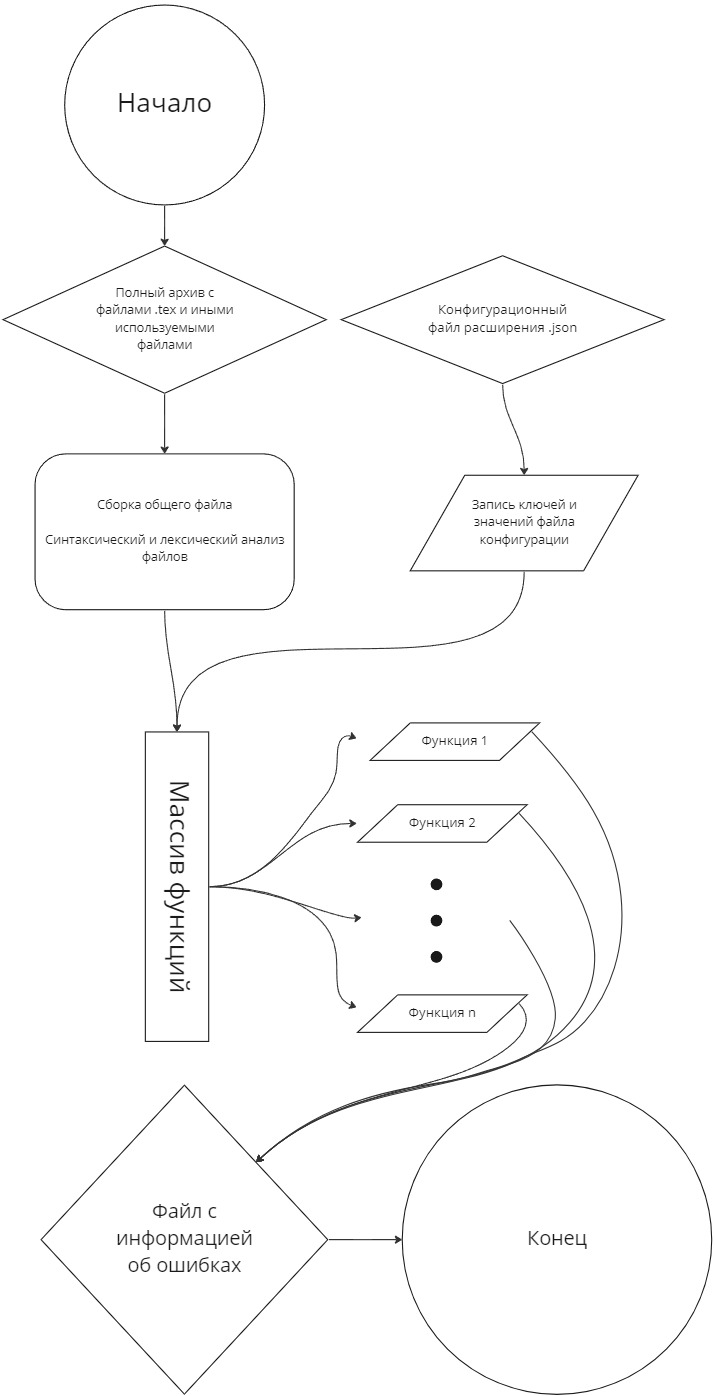
\includegraphics[width=12cm]{Images/WorkToGo.png}
        \caption{Общая схема работы программы}
        \label{fig:3}
    \end{figure}
